\documentclass[12pt,a4paper]{article}
\usepackage[utf8]{inputenc}
\usepackage[spanish]{babel}
\usepackage{graphicx}
\usepackage{url}
\usepackage[breaklinks=true]{hyperref}
\usepackage{listings}
\usepackage{color}
\usepackage{booktabs}
\usepackage{longtable}
\usepackage{array}
\usepackage[margin=2.5cm]{geometry}
\usepackage{microtype}
\usepackage{xspace}

% Evitar problemas de overfull hbox
\sloppy
\setlength{\emergencystretch}{3em}
\hyphenpenalty=10000
\exhyphenpenalty=10000

% Configuración para código fuente
\definecolor{codegray}{rgb}{0.5,0.5,0.5}
\definecolor{codepurple}{rgb}{0.58,0,0.82}
\definecolor{codeback}{rgb}{0.95,0.95,0.95}
\lstdefinestyle{mypython}{
    backgroundcolor=\color{codeback},   % color de fondo
    commentstyle=\color{green!50!black},
    keywordstyle=\color{blue},
    numberstyle=\tiny\color{codegray},
    stringstyle=\color{codepurple},
    basicstyle=\ttfamily\small,
    breakatwhitespace=false,
    breaklines=true,
    captionpos=b,
    keepspaces=true,
    numbers=left,
    numbersep=5pt,
    showspaces=false,
    showstringspaces=false,
    showtabs=false,
    tabsize=2
}
\lstdefinestyle{myjavascript}{
    backgroundcolor=\color{codeback},
    commentstyle=\color{green!50!black},
    keywordstyle=\color{blue},
    numberstyle=\tiny\color{codegray},
    stringstyle=\color{codepurple},
    basicstyle=\ttfamily\small,
    breaklines=true,
    numbers=left,
    numbersep=5pt,
    showstringspaces=false
}

\title{Documentación del Proyecto: Analizador LR(1)}
\author{Puntos Extras Examen 2 \\ Curso de Compiladores \\ Universidad de Ingeniería y Tecnología (UTEC)}
\date{Octubre 2024}

\begin{document}
\maketitle
\tableofcontents
\newpage

\section{Introducción}

Este documento describe de manera detallada la implementación de un \emph{analizador sintáctico LR(1)} desarrollado como parte de los puntos extras del Examen~2 del curso de Compiladores de la UTEC.  El proyecto implementa un parser LR(1) desde cero y provee una interfaz web moderna construida con React.  La aplicación es capaz de leer gramáticas libres de contexto, construir el autómata LR(1) canónico, generar la tabla de análisis \texttt{ACTION}/\texttt{GOTO} y analizar cadenas de entrada mostrando la traza completa del proceso.  Además, incluye visualizaciones profesionales del autómata mediante \texttt{Graphviz}.

\subsection{Objetivos}
\begin{itemize}
  \item Implementar un parser LR(1) canónico desde cero, superando los requisitos del proyecto (que solicitaba un LALR(1)).
  \item Proporcionar una interfaz web intuitiva para interactuar con el parser y visualizar resultados.
  \item Permitir la visualización del autómata LR(1) y de la tabla de análisis de manera clara y profesional.
  \item Facilitar el análisis de cadenas con trazabilidad paso a paso.
  \item Soportar sintaxis con el operador ``|'' para especificar múltiples producciones en una sola línea.
\end{itemize}

\section{Fundamentos teóricos}

\subsection{Parsers LR(1)}

El término LR(1) significa \textbf{L}eft-to-right parsing con construcción de una derivación por la \textbf{R}everse rightmost derivation y utilizando un símbolo de \textbf{lookahead}.  Los parsers LR(1) son capaces de analizar un superconjunto de gramáticas que las variantes SLR(1) o LALR(1); aunque generan más estados, resuelven más conflictos \emph{shift}/\emph{reduce} y \emph{reduce}/\emph{reduce}.  Utilizan un \emph{item LR(1)} de la forma $[A \to \alpha\bullet\beta, a]$, donde $a$ es el \emph{lookahead}.  Cada item indica que se ha visto la parte $\alpha$ de la producción y se espera leer $\beta$ con $a$ como símbolo de anticipación.

\subsection{Componentes clave}

Un parser LR(1) se construye a partir de los siguientes componentes:

\begin{itemize}
  \item \textbf{Conjuntos FIRST}.  Para cada símbolo se determina el conjunto de terminales con los que puede comenzar cualquier derivación; permiten calcular \emph{lookaheads} correctos.
  \item \textbf{Conjuntos FOLLOW}.  Para cada no terminal se determina el conjunto de terminales que pueden aparecer inmediatamente a su derecha; se utilizan en la construcción de las reglas de reducción.
  \item \textbf{Items LR(1)}.  Expresan el progreso en una producción y el lookahead permitido.
  \item \textbf{Función \texttt{closure}}.  Calcula la clausura de un conjunto de items, añadiendo nuevos items cuando el punto se encuentra antes de un no terminal, propagando correctamente los \emph{lookaheads}.
  \item \textbf{Función \texttt{goto}}.  Calcula la transición al avanzar el punto sobre un símbolo; define las transiciones del autómata.
  \item \textbf{Tablas ACTION y GOTO}.  Determinan, para cada estado y símbolo, si la acción es desplazar, reducir, aceptar o error, y a qué estado transicionar después de una reducción.
\end{itemize}

\subsection{Algoritmo de construcción}

A continuación se describe de forma resumida el algoritmo para construir un parser LR(1).  La construcción utiliza un algoritmo de punto fijo para calcular los conjuntos \texttt{FIRST} y \texttt{FOLLOW}, tras lo cual se construye el autómata canónico y las tablas de análisis.

\begin{enumerate}
  \item Calcular los conjuntos FIRST y FOLLOW para todos los símbolos de la gramática.
  \item Crear una \emph{gramática aumentada} añadiendo una producción $S' \to S$ donde $S$ es el símbolo inicial original.
  \item Construir el autómata LR(1): se toma como estado inicial $\texttt{closure}(\{[S' \to \bullet S, \$]\})$ y se generan sucesivos estados aplicando \texttt{goto} sobre todos los símbolos posibles; cada nuevo conjunto de items genera un nuevo estado.
  \item Construir las tablas ACTION y GOTO: para cada estado y símbolo se asigna una acción de desplazamiento, reducción o aceptación según la posición del punto y el lookahead en los items.
  \item Utilizar las tablas para analizar cadenas; se emplea una pila de estados y un apuntador de entrada, desplazando y reduciendo conforme lo indique la tabla ACTION.
\end{enumerate}

\section{Arquitectura del proyecto}

El proyecto se divide en tres módulos principales: el backend en Python, el parser propiamente dicho (implementado en un paquete \texttt{parser/}) y el frontend en React.  La tabla~\ref{tab:estructura} muestra la estructura de directorios.

\begin{table}[h]
\centering
\begin{tabular}{ll}
\toprule
\textbf{Directorio} & \textbf{Descripción} \\
\midrule
\texttt{backend/} & API REST con Flask\\
\texttt{frontend/react-app/} & Aplicación React + Vite\\
\texttt{parser/} & Implementación del parser LR(1)\\
\texttt{requirements.txt} & Dependencias Python\\
\texttt{README.md} & Documentación de usuario\\
\bottomrule
\end{tabular}
\caption{Estructura general del proyecto.}
\label{tab:estructura}
\end{table}

\subsection{Backend}

El backend está construido con \textbf{Flask~3.0.0} y expone una API REST para construir el parser, generar visualizaciones y analizar cadenas.  El archivo \texttt{app.py} define los siguientes endpoints principales:
\begin{itemize}
  \item \texttt{/api/build\_parser} (POST): recibe una gramática, construye el parser e informa sobre el autómata (número de estados y transiciones, terminales, no terminales, producciones y conjuntos FIRST/FOLLOW).
  \item \texttt{/api/parse\_string} (POST): recibe una cadena de entrada y devuelve si es aceptada junto con la traza de análisis.
  \item \texttt{/api/generate\_graphviz} (POST): genera una representación visual del autómata en formato \texttt{SVG} y \texttt{PNG} mediante Graphviz.
  \item \texttt{/api/get\_parsing\_table} (GET): devuelve la tabla ACTION/GOTO completa para inspección o visualización.
\end{itemize}
El backend utiliza las clases implementadas en \texttt{parser/lr1\_parser.py} para procesar la gramática y analizar cadenas.  Para la visualización se hace uso de \texttt{graphviz} y \texttt{networkx}, y se soporta \texttt{CORS} para permitir el consumo desde el frontend.

\subsection{Parser}

El núcleo del proyecto se encuentra en el paquete \texttt{parser/}.  La clase central es \texttt{LR1Parser}, implementada en \texttt{lr1\_parser.py}, que encapsula toda la lógica de construcción del parser LR(1).  A continuación se muestran algunos de sus elementos más importantes (extracto):

\begin{lstlisting}[style=mypython, language=Python, caption={Definición de clases y atributos principales del parser.}]
from dataclasses import dataclass, field
from typing import List, Set, Dict, Tuple

@dataclass
class Production:
    """Representa una producción de la gramática"""
    left: str
    right: List[str]
    number: int = 0

@dataclass
class LR1Item:
    """Representa un item LR(1) con lookahead"""
    production: int
    dot_position: int
    lookahead: str

class LR1Parser:
    """Parser LR(1) completo"""
    def __init__(self):
        self.grammar: List[Production] = []
        self.terminals: Set[str] = set()
        self.non_terminals: Set[str] = set()
        self.first_sets: Dict[str, Set[str]] = {}
        self.follow_sets: Dict[str, Set[str]] = {}
        self.states: List[Set[LR1Item]] = []
        self.transitions: Dict[Tuple[int,str], int] = {}
        self.action_table: Dict[Tuple[int,str], str] = {}
        self.goto_table: Dict[Tuple[int,str], int] = {}
\end{lstlisting}

El método \texttt{\_compute\_first\_sets()} implementa el cálculo de los conjuntos FIRST mediante un algoritmo de punto fijo, mientras que \texttt{\_compute\_follow\_sets()} calcula los conjuntos FOLLOW.  Posteriormente \texttt{\_build\_lr1\_automaton()} genera los estados del autómata aplicando clausura y transiciones y \texttt{\_build\_parsing\_table()} construye las tablas ACTION y GOTO.  El método \texttt{parse\_string()} emplea las tablas para analizar cadenas, manteniendo una pila de estados y una traza de pasos.

\subsection{Frontend}

La interfaz de usuario está construida con \textbf{React~18} y utiliza \texttt{Vite} como herramienta de construcción y servidor de desarrollo.  Los componentes principales son:
\begin{itemize}
  \item \texttt{GrammarEditor.jsx}: permite ingresar una gramática, cargar ejemplos y solicitar la construcción del parser.  Utiliza un área de texto con estado interno y un botón que invoca la API REST.
  \item \texttt{AutomatonInfo.jsx}: muestra información resumida del autómata (número de estados, transiciones, terminales y no terminales) en tarjetas.
  \item \texttt{VisualizationTabs.jsx}: organiza en pestañas la visualización Graphviz y la tabla ACTION/GOTO.  Al cambiar de pestaña se realizan peticiones a la API para obtener la última versión de la visualización.
  \item \texttt{StringParser.jsx}: permite ingresar una cadena de entrada y consultar si es aceptada, mostrando además la traza de análisis en una tabla.
\end{itemize}
A modo de ejemplo, el código de \texttt{GrammarEditor.jsx} luce así:

\begin{lstlisting}[style=myjavascript, language=JavaScript, caption={Componente para editar y construir la gramática.}]
function GrammarEditor({ onBuild, loading, error }) {
  const [grammar, setGrammar] = useState(DEFAULT_GRAMMAR);

  const handleBuild = () => {
    onBuild(grammar);
  };

  return (
    <div className="section">
      <h2>Gramática</h2>
      <textarea
        value={grammar}
        onChange={(e) => setGrammar(e.target.value)}
        rows={10}
      />
      <button onClick={handleBuild} disabled={loading}>
        {loading ? 'Construyendo...' : 'Construir Parser'}
      </button>
      {error && <div className="alert alert-error">{error}</div>}
    </div>
  );
}
\end{lstlisting}

\section{Instalación y uso de la aplicación}

\subsection{Requisitos previos}

Para ejecutar la aplicación se requiere tener instalado lo siguiente:
\begin{itemize}
  \item Python 3.9 o superior
  \item Node.js 18 o superior
  \item npm 9 o superior
  \item Graphviz (instalado en el sistema)
\end{itemize}

\subsection{Instalación de Graphviz}

Graphviz debe instalarse en el sistema operativo antes de ejecutar la aplicación:

\begin{verbatim}
# macOS
brew install graphviz

# Linux (Ubuntu/Debian)
sudo apt-get install graphviz

# Windows
# Descargar desde https://graphviz.org/download/
\end{verbatim}

\subsection{Instalación de dependencias}

\textbf{Dependencias de Python:}
\begin{verbatim}
pip3 install -r requirements.txt
\end{verbatim}

Las dependencias incluidas son:
\begin{itemize}
  \item Flask 3.0.0
  \item Flask-CORS 4.0.0
  \item matplotlib 3.8.2
  \item networkx 3.2.1
  \item graphviz $\geq$ 0.16
  \item Pillow $\geq$ 10.1.0
\end{itemize}

\textbf{Dependencias de React:}
\begin{verbatim}
cd frontend/react-app
npm install
cd ../..
\end{verbatim}

\subsection{Ejecución de la aplicación}

La aplicación consta de dos componentes que deben ejecutarse en terminales separadas:

\textbf{Backend (Terminal 1):}
\begin{verbatim}
python3 -m backend.app
\end{verbatim}

El backend estará disponible en \url{http://localhost:5001}

\textbf{Frontend (Terminal 2):}
\begin{verbatim}
cd frontend/react-app
npm run dev
\end{verbatim}

El frontend estará disponible en \url{http://localhost:5173}

\subsection{Funciones de la interfaz}

\begin{itemize}
  \item \textbf{Editor de gramáticas}.  Permite escribir gramáticas libres de contexto, separando símbolos con espacios y utilizando $\varepsilon$ o \texttt{epsilon} para producciones vacías.  Además, soporta el uso del operador ``|'' para especificar múltiples alternativas en una sola línea (por ejemplo, \texttt{C -> a | b}).
  \item \textbf{Construcción del parser}.  Al pulsar «Construir Parser» se envía la gramática al backend; el sistema responde con el número de estados, transiciones y los conjuntos FIRST y FOLLOW.
  \item \textbf{Visualización del autómata}.  La pestaña «Graphviz» muestra los items LR(1) con sus lookaheads.  La visualización incluye una transición especial con el símbolo \$ hacia un estado final marcado como ACCEPT.
  \item \textbf{Tabla ACTION/GOTO}.  Permite inspeccionar la tabla de análisis completa; las acciones \texttt{shift}, \texttt{reduce} y \texttt{accept} se colorean para mayor claridad.
  \item \textbf{Análisis de cadenas}.  Permite ingresar una cadena y conocer si es aceptada; se presenta la traza paso a paso con la pila de estados, la entrada restante y la acción tomada.
\end{itemize}

\section{Ejemplos y resultados}

Se incluye a continuación un ejemplo de gramática y los conjuntos FIRST y FOLLOW correspondientes, además de un ejemplo de traza de análisis.  Esta información sirve para comprobar el funcionamiento del parser.

\subsection{Gramática de ejemplo}

\begin{verbatim}
S -> q * A * B * C
A -> a
A -> b * b * D
B -> a | ε
C -> b | ε
D -> C | ε
\end{verbatim}

Nótese el uso del operador ``|'' para especificar alternativas en las producciones de B, C y D.

\subsection{Conjuntos FIRST}

\begin{table}[h]
\centering
\begin{tabular}{lr}
\toprule
Símbolo & FIRST( ) \\
\midrule
$S$ & $\{q\}$ \\
$A$ & $\{a, b\}$ \\
$B$ & $\{a, \epsilon\}$ \\
$C$ & $\{b, \epsilon\}$ \\
$D$ & $\{b, \epsilon\}$ \\
\bottomrule
\end{tabular}
\caption{Conjuntos FIRST del ejemplo.}
\end{table}

\subsection{Conjuntos FOLLOW}

\begin{table}[h]
\centering
\begin{tabular}{lr}
\toprule
Símbolo & FOLLOW( ) \\
\midrule
$S$ & $\{\$\}$ \\
$A$ & $\{*\}$ \\
$B$ & $\{*\}$ \\
$C$ & $\{\$, *\}$ \\
$D$ & $\{*\}$ \\
\bottomrule
\end{tabular}
\caption{Conjuntos FOLLOW del ejemplo.}
\end{table}

\subsection{Información del autómata}

Para la gramática anterior se obtienen 19 estados y 18 transiciones.  El autómata reconoce cinco terminales ($\$$, $*$, $a$, $b$, $q$) y seis no terminales ($S$, $S'$, $A$, $B$, $C$, $D$).  La tabla ACTION/GOTO generada tiene 19 filas (estados) y columnas para cada símbolo.  La figura~\ref{fig:automata} ilustra un ejemplo de visualización del autómata mediante Graphviz.

% Se asume que el archivo automata_graphviz.svg está disponible en la carpeta de static; se puede reemplazar la ruta si se cambia de ubicación.
\begin{figure}[h]
\centering
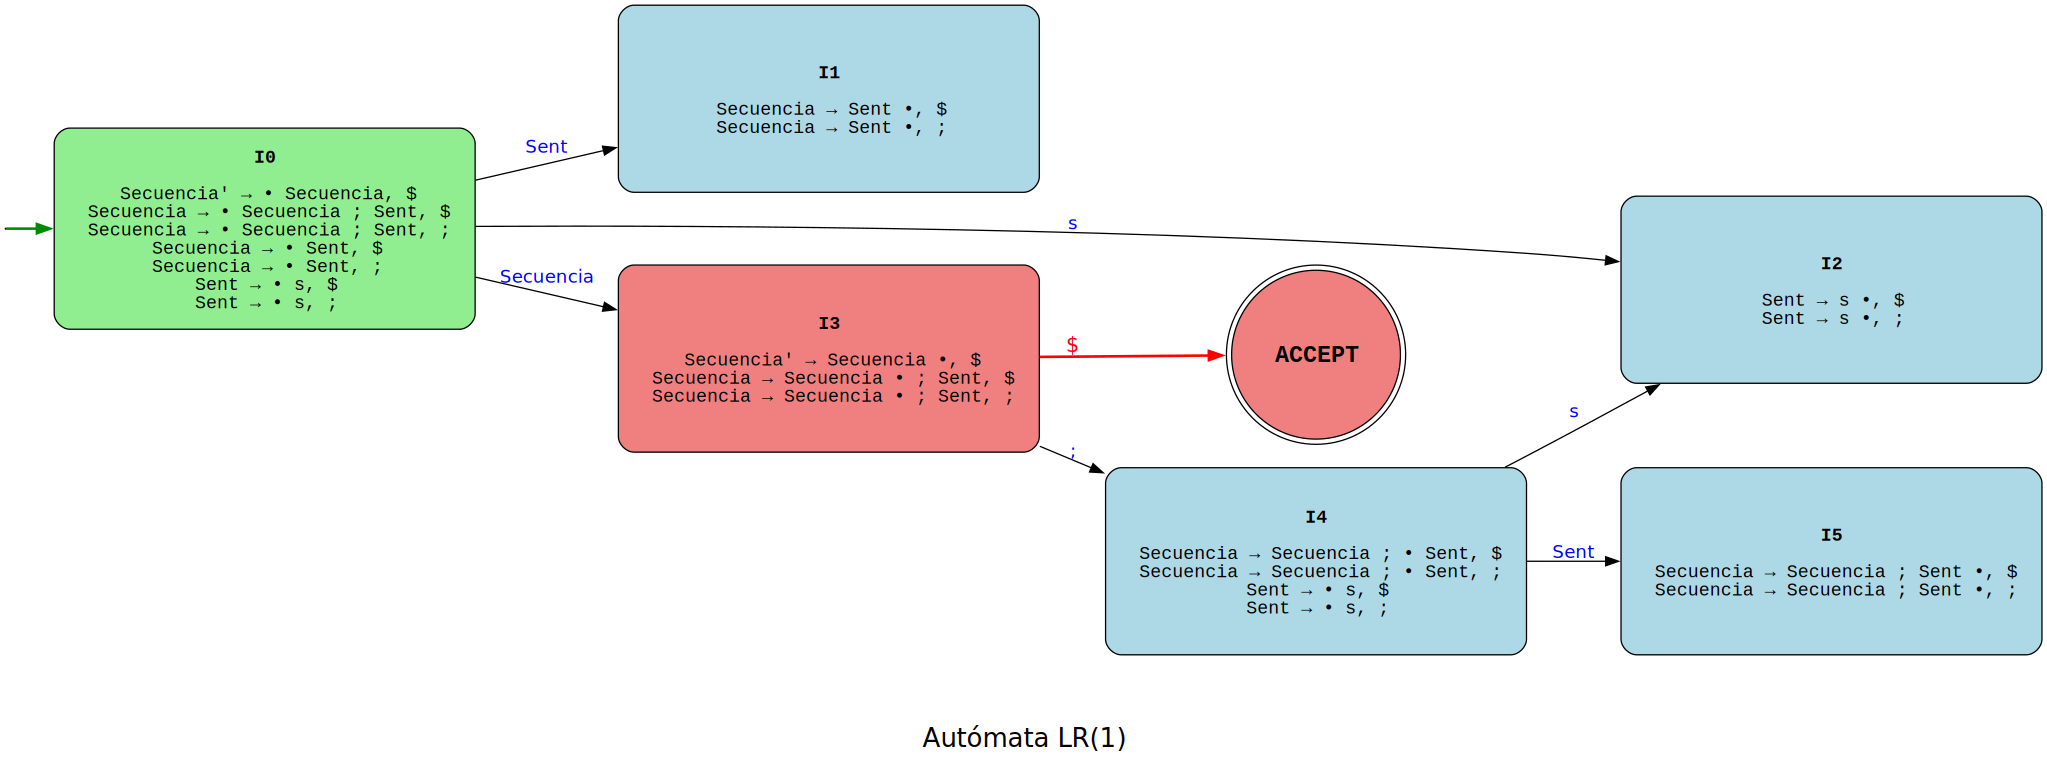
\includegraphics[width=0.9\textwidth]{frontend/static/automata_graphviz}
\caption{Vista del autómata LR(1) generado con Graphviz para la gramática de ejemplo. Nótese la transición con \$ hacia el estado ACCEPT.}
\label{fig:automata}
\end{figure}

\subsection{Traza de análisis de cadena}

A continuación se muestra la traza generada al analizar la cadena \texttt{q * a * a * b}, donde cada fila indica el contenido de la pila, la entrada restante y la acción tomada:

\begin{longtable}{lll p{5cm}}
\toprule
Paso & Pila & Entrada & Acción \\
\midrule
1 & 0 & $q * a * a * b \$ $ & shift 1 \\
2 & 0\,1 & $* a * a * b \$ $ & shift 3 \\
3 & 0\,1\,3 & $a * a * b \$ $ & shift 4 \\
4 & 0\,1\,3\,4 & $* a * b \$ $ & reduce 2 ($A \to a$) \\
5 & 0\,1\,3\,5 & $* a * b \$ $ & shift 7 \\
6 & 0\,1\,3\,5\,7 & $a * b \$ $ & shift 10 \\
7 & 0\,1\,3\,5\,7\,10 & $* b \$ $ & reduce 4 ($B \to a$) \\
8 & 0\,1\,3\,5\,7\,12 & $* b \$ $ & shift 13 \\
9 & 0\,1\,3\,5\,7\,12\,13 & $b \$ $ & shift 14 \\
10 & 0\,1\,3\,5\,7\,12\,13\,14 & $\$ $ & reduce 6 ($C \to b$) \\
11 & 0\,1\,3\,5\,7\,12\,13\,15 & $\$ $ & reduce 1 ($S \to q * A * B * C$) \\
12 & 0\,2 & $\$ $ & ACCEPT \\
\bottomrule
\end{longtable}

\section{Características destacadas}

El proyecto presenta varias funcionalidades que exceden los requisitos del examen:
\begin{itemize}
  \item \textbf{Parser LR(1) completo}.  Se implementa un algoritmo LR(1) canónico en lugar de LALR(1), con cálculo correcto de lookaheads, manejo de producciones \emph{epsilon} y construcción de tablas ACTION/GOTO.
  \item \textbf{Soporte para sintaxis con alternativas}.  El parser reconoce el operador ``|'' para especificar múltiples producciones en una sola línea, simplificando la escritura de gramáticas.
  \item \textbf{Visualización profesional con Graphviz}.  Se generan visualizaciones detalladas que muestran los items LR(1) completos con lookaheads, estados coloreados (verde para inicial, rojo para aceptación) y una transición explícita con \$ hacia el estado ACCEPT.
  \item \textbf{Interfaz web moderna}.  La aplicación utiliza React con arquitectura de componentes y proporciona una experiencia de usuario fluida; la tabla ACTION/GOTO se colorea según el tipo de acción.
  \item \textbf{Manejo de errores}.  El backend valida gramáticas y cadenas, devolviendo mensajes descriptivos; la traza de análisis se detiene en caso de error sintáctico.
\end{itemize}

\section{Comparación con los requisitos}

Se presenta a continuación una comparación entre los requisitos del proyecto y las funcionalidades implementadas.

\begin{table}[h]
\centering
\begin{tabular}{p{4cm} p{3cm} p{8cm}}
\toprule
\textbf{Requisito} & \textbf{Estado} & \textbf{Detalles} \\
\midrule
Parser LALR(1) & Superado & Se implementó un LR(1) canónico, más potente que LALR(1). \\
Interfaz gráfica & Cumplido & Aplicación React con secciones para gramática, autómata, tabla y análisis de cadenas. \\
Reporte pequeño & Cumplido & Este documento incluye una explicación completa del proyecto. \\
Uso exclusivo de Python & Cumplido & El backend está escrito en Python; el frontend se implementó adicionalmente para mejorar la experiencia. \\
Presentación & Cumplido & El proyecto cuenta con visualización en vivo del autómata y de las tablas de análisis. \\
\bottomrule
\end{tabular}
\caption{Estado de los requisitos del proyecto.}
\end{table}

\section{Limitaciones y trabajo futuro}

Aunque el parser LR(1) implementado es completo y funcional, existen limitaciones que podrían abordarse en versiones posteriores:
\begin{itemize}
  \item \textbf{Detección de ambigüedad}.  El sistema no detecta automáticamente si una gramática es ambigua; en caso de conflictos toma la primera acción disponible.
  \item \textbf{Minimización de estados}.  No se ha implementado la fusión de estados típica de LALR(1); por ello se generan más estados que los necesarios.
  \item \textbf{Rendimiento de visualización}.  Para gramáticas grandes, la visualización con Graphviz puede ser lenta y producir diagramas extensos.
  \item \textbf{Optimización del algoritmo}.  La construcción del autómata podría paralelizarse o guardarse en caché para gramáticas repetidas.
\end{itemize}

En cuanto al trabajo futuro se proponen las siguientes mejoras:
\begin{itemize}
  \item Implementar detección de conflictos \emph{shift}/\emph{reduce} y \emph{reduce}/\emph{reduce}, así como la conversión a LALR(1).
  \item Integrar un editor con resaltado de sintaxis y un modo oscuro en la interfaz web.
  \item Permitir exportar la tabla de análisis a diferentes formatos y generar código de parser a partir de la tabla.
  \item Añadir un histórico de gramáticas y la posibilidad de compartirlas mediante enlaces.
\end{itemize}

\section{Conclusiones}

Se ha desarrollado un analizador sintáctico LR(1) completo y se ha integrado con una interfaz web moderna, superando ampliamente los requisitos iniciales del proyecto.  El parser maneja adecuadamente producciones vacías, soporta sintaxis con alternativas mediante el operador ``|'', y genera lookaheads precisos, produciendo tablas ACTION/GOTO correctas.  La arquitectura modular del código facilita la reutilización y el mantenimiento.  Este proyecto no sólo demuestra conocimientos teóricos de análisis sintáctico, sino que también integra conceptos de desarrollo full-stack, y puede servir como base para diseñar lenguajes de programación o validar gramáticas en contextos académicos y profesionales.

\section{Referencias}

\begin{enumerate}
  \item Aho, A. V., Lam, M. S., Sethi, R., \& Ullman, J. D. \textit{Compilers: Principles, Techniques, and Tools} (2nd ed.). Pearson, 2006.
  \item Cooper, K., \& Torczon, L. \textit{Engineering a Compiler} (2nd ed.). Morgan Kaufmann, 2011.
  \item Appel, A. W. \textit{Modern Compiler Implementation in ML}. Cambridge University Press, 2004.
  \item Documentación oficial de Python: \url{https://docs.python.org/3/}
  \item Documentación de React: \url{https://react.dev/}
  \item Documentación de Flask: \url{https://flask.palletsprojects.com/}
  \item Documentación de Graphviz: \url{https://graphviz.org/documentation/}
\end{enumerate}

\end{document}
